\documentclass[12pt]{article}

\usepackage{../header}
\newcommand{\mbf}{\mathbf}
\newcommand{\A}{\; \forall \;}
\newcommand{\E}{\; \exists \;}
\usepackage{subcaption}

% Node styles
\tikzstyle{operator_node}=[fill={rgb,255: red,0; green,185; blue,242}, draw=black, shape=circle]
\tikzstyle{tensor_node}=[fill={rgb,255: red,255; green,159; blue,43}, draw=black, shape=circle]

\begin{document}
    \section*{Подготовительный этап: на пути к отношению Реллея}
    \subsection*{Основные определения}
    \begin{definition}
        \it{Тензорным (полилинейным) отображением} будем называть отображение\\ $\mathcal{A} \colon\RR^{n_1 \times n_2 \times \ldots \times n_d} \to \RR^{m_1 \times m_2 \times \ldots \times m_d}$,
        линейное по каждому аргументу, при фиксированных прочих.
    \end{definition}
    Такое отображение (при фиксированных базисах) можно задать тензором $\mbf{A} \in \RR^{(m_1 \times n_1) \times \ldots \times (m_d \times n_d)}$,
    причём $\A V \in \RR^{m_1 \times m_2 \times \ldots \times m_d} \E T \in \RR^{n_1 \times n_2 \times \ldots \times n_d}$ такой что
    \[
        V = \mathcal{A}(T) = \mbf{A} \cdot T
    \]
    где умножение тензорного оператора $\mbf{A}$ на тензор $T$ осуществляется по правилу
    \begin{align}
    (\mbf{A} \cdot T)
        _{i_1, \ldots, i_d} = \sum_{j_1 = 1}^{n_1}\cdots\sum_{j_d = 1}^{n_d} \mbf{A}_{i_1, j_1, \ldots, i_d, j_d} \cdot T_{j_1, \ldots, j_d}
    \end{align}
    \begin{comment}
        Если source и target пространства совпадают, то будем называть $\mathcal{A}$ тензорным (полилинейным) оператором.
    \end{comment}
    \begin{definition}
        \it{Собственными значениями} тензорного оператора $\mathcal{A}$ называются значения $\lambda \in \RR$, удовлетворяющие уравнению
        \[
            \mathcal{A}(T) = \lambda T
        \]
        Соответствующие $T \in \RR^{n_1 \times n_2 \times \ldots \times n_d} \setminus \{0\}$ называются \it{собственными тензорами}.
    \end{definition}
    \begin{definition}
        Тензорный оператор $\mathcal{A}$, задаваемый тензором $\mbf{A}$ называется \it{симметричным}, если
        $\A (i_1, \ldots, i_d) \subset \NN^{d}, (j_1, \ldots, j_d) \subset \NN^{d}$
        выполнено
        \[
            \mbf{A}_{i_1, j_1, \ldots, i_d, j_d} = \mbf{A}_{j_1, i_1, \ldots, j_d, i_d}
        \]
    \end{definition}
    \begin{definition}
        \it{Скалярным произведением тензоров} называется симметричная, полилинейная форма
        $(\cdot, \cdot)\colon \RR^{n_1 \times n_2 \times \ldots \times n_d} \times \RR^{n_1 \times n_2 \times \ldots \times n_d} \to \RR$,
        по правилу
        \[
            (X, Y) \mapsto \sum_{i_1, \ldots, i_d} X_{i_1, \ldots, i_d} Y_{i_1, \ldots, i_d}
        \]
        Здесь положительная определённость понимается в обычном смысле: $X \in \RR^{n_1 \times n_2 \times \ldots \times n_d}\setminus \{0\} \implies (X, X) > 0$.
    \end{definition}
    \subsection*{Постановка задачи}
    Аналогично с матричным случаем, можно определить отношение Реллея следующим образом: если симметричный тензорный оператор
    $\mathcal{A} \colon\RR^{n_1 \times n_2 \times \ldots \times n_d} \to \RR^{n_1 \times n_2 \times \ldots \times n_d}$ задаётся тензором $\mbf{A}$,
    то отношение Реллея:
    \[
        R(T) = \frac{(T, \mbf{A}T)}{(T, T)}
    \]
    Так же аналогично с матричным случаем выполнено
    \begin{align*}
        &\min \lambda_i = \min_{T \neq 0} R(T)
        &&\max \lambda_i = \max_{T \neq 0} R(T)
    \end{align*}
    Эти значения могут быть найдены методами Римановой оптимизации (даже понятно, что конкретно надо делать). В чём же проблема? А проблем на самом деле
    несколько:
    \begin{enumerate}
        \item В пакете TTAX не реализовано умножение тензора на тензор;
        \item Не ясно, откуда брать симметричные тензоры (кроме супердиагональных);
    \end{enumerate}
    На практике вторая проблема наверняка и не проблема вовсе: я просто ещё не искал, как делать симметричные тензоры (понятно, что можно просто
    сделать $\mbf{A}^T\mbf{A}$, это не интересно). Первая проблема куда более серьёзная, ей и будем заниматься.
    \subsection*{Тензорный матвек}
    Чего мы в сущности ждём от операции, которую хотим реализовать? Запишем все наши желания для функции, реализующей операцию:
    \begin{itemize}
        \item Функция принимает два тензора в формате ТТ, один из которых --- оператор;
        \item Функция нигде не должна собирать тензор целиком;
        \item Функция выполняет умножение оператора на тензор и возвращает ответ в ТТ формате;
        \item В функции не должно быть никаких side-эффектов, чтобы не мешать автодифференцированию;
    \end{itemize}
    \begin{definition}
        Говорят, что тензор $T \in \RR^{n_1 \times n_2 \times \ldots \times n_d}$ имеет \it{TT-разложение}
        $\left[ T^{(1)}, \ldots, T^{(d)} \right]$, если каждый его элемент может быть представлен в виде
        \[
            T_{i_1, \ldots, i_d} = \sum_{k_0 = 1}^{r_0} \cdots \sum_{k_d = 1}^{r_d} T^{(1)}_{k_0, i_1, k_1} \cdot\ldots\cdot T^{(d)}_{k_{d-1}, i_d, k_d}
        \]
        Тензоры $T^{(i)} \in \RR^{r_{i-1} \times n_i \times r_i}$ называются \it{TT-ядрами}, а вектор $(r_1, \ldots, r_{d-1})$ называется \it{TT-рангом}.
    \end{definition}
    Кроме того мы будем представлять TT-разложение тензора $T$ в виде тензорной сети следующим образом:
    \begin{center}
        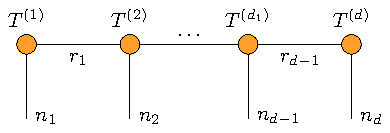
\includegraphics[scale=1.2]{./pic/tensornet_tensor}
    \end{center}

    \begin{definition}
        Будем говорить, что тензорный оператор $\mbf{A} \in \RR^{(m_1 \times n_1) \times \ldots \times (m_d \times n_d)}$ имеет \it{TT-разложение}
        $\left[ A^{(1)}, \ldots, A^{(d)} \right]$, если каждый его элемент может быть представлен в виде
        \[
            \mbf{A}_{i_1, j_1, \ldots, i_d, j_d} = \sum_{k_0 = 1}^{r_0} \cdots \sum_{k_d = 1}^{r_d} A^{(1)}_{k_0, i_1, j_1, k_1} \cdot\ldots\cdot A^{(d)}_{k_{d-1}, i_d, j_d, k_d}
        \]
        Соответственно тензоры $A^{(i)} \in \RR^{r_{i-1} \times m_i \times n_i \times r_i}$ --- его \it{TT-ядра}, вектор $(r_1, \ldots, r_{d-1})$ --- его \it{TT-ранг}.
    \end{definition}
    \begin{definition}
        По соглашению значения $r_0$ и $r_d$ полагаются равными $1$.
    \end{definition}
    Будем представлять TT-разложение оператора $\mbf{A}$ в виде тензорной сети следующим образом:
    \begin{center}
        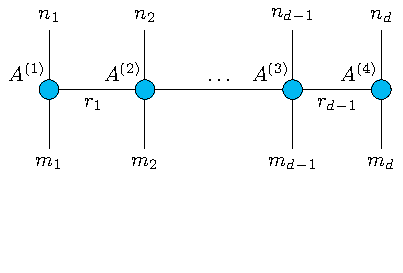
\includegraphics[scale=1.2]{./pic/tensornet_operator}
    \end{center}
    Сразу можно заметить ещё одну проблему: мы хотим, чтобы TT-ядра оператора являлись тензорами четвёртого порядка, в то время как TTAX
    позволяет нам хранить в ядрах только тензоры порядка $3$. Чтобы решить эту проблему, опишем процедуру получения TT-разложения оператора с ядрами
    четвёртого порядка, имея на руках ТТ-разложение оператора с ядрами третьего порядка:

    Сейчас тензорный оператор $\mbf{A} \in \RR^{m_1 \times n_1 \times \ldots \times m_d \times n_d}$ представляется в
    TTAX в виде $\left[ A^{(1)}, \ldots, A^{(2d)} \right]$, где $A^{(k)} \in \RR^{r_{k - 1} \times m_k \times r_k}$, а
    $A^{(k+1)} \in \RR^{r_{k} \times n_k \times r_{k+1}}$. Имея два таких тензора порядка $3$ мы можем свернуть их по общей моде и получить тензор порядка $4$.
    Нагляднее покажем процесс на тензорной сети:
    \begin{figure}[h!]
        \centering
        \begin{subfigure}[b]{0.47\linewidth}
            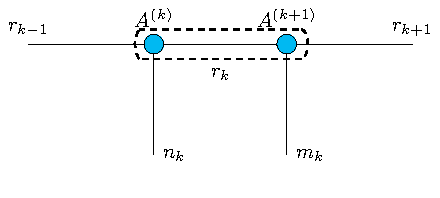
\includegraphics[width=\linewidth]{./pic/tensornet_operator_2cores}
            \caption{Два ядра порядка $3$ до свёртки}
        \end{subfigure}
        \begin{subfigure}[b]{0.33\linewidth}
            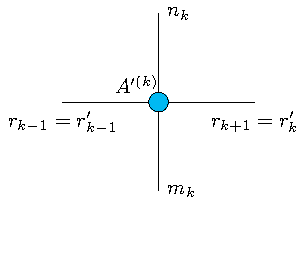
\includegraphics[width=\linewidth]{./pic/tensornet_operator_1core}
            \caption{Полученное ядро порядка $4$}
        \end{subfigure}
    \end{figure}

    Таким образом мы описали процедуру, как имея TT-разложение оператора в формате, предоставляемом TTAX получить TT-разложение в нужном нам формате.

    Теперь рассмотрим операцию произведения тензорного оператора $\mbf{A} \in \RR^{(m_1 \times n_1) \times \ldots \times (m_d \times n_d)}$
    на тензор $T \in \RR^{n_1 \times \ldots \times n_d}$. Если расписать формулу $(1)$, подставив на места тензоров $\mbf{A}$ и $T$ соответствующие им
    TT-разложения, то станет ясно, что один и тот же индекс, по которому ведётся суммирование (скажем, $j_k$), встречается один раз в $A^{(k)}$,
    и один раз в $T^{(k)}$, и больше не встречается. Это значит, что произведение оператора на тензор может быть записано в терминах произведения
    конкретных TT-ядер. Покажем процесс произведения оператора на тензор наглядно через тензорные сети:

    \begin{figure}
        \centering
        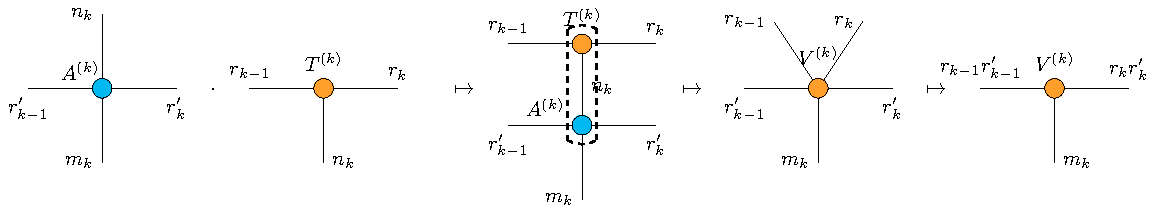
\includegraphics[scale=0.92]{./pic/tensornet_product}
        \caption{Процесс умножения оператора на тензор $V = \mbf{A}\cdot T$}
    \end{figure}

    Осталось это только заимплементить, и можно приступать к Римановой оптимизации.
\end{document}